The full analysis is performed on 188 $\pm$ 8 $\ipb$ of integrated luminosity, as a 
preparation for larger luminosity scenarios in the near future.

\subsection{Background Expectation in the $\WW$ Region}
The estimation of the backgrounds follows the strategies described in 
Section~\ref{sec:backgrounds}. We summarize here the yields for the main background
components. For $\dyll$, top and $\Wjets$ backgrounds, we report the 
expected yields after the $\WW$ selection, those results are then extrapolated 
to each Higgs signal mass point.

The expected contributions from $\dyll$ events outside the $Z$-mass region in data 
is estimated in a data-driven techinque described in Section~\ref{sec:bkg_dy}. 
This procedure is applied separately to electrons and muons in all jet bins. 
The predictions for the off-peak $\dymm+X$ and $\dyee+X$ contributions 
using the 188 $\ipb$ data are tablulated in Tables~\ref{tab:dyestmm} and~\ref{tab:dyestee} respectively. 

%%%%%%%%%%%%%%%%%%%%%%%%%%%%%%
\begin{table}
\begin{center}
\begin{tabular}{l c c c}
\hline
Sample                                 &   0-jet             & 1-jet & 2-jet        \\
\hline
$R_{out/in}$ (simulation)              &   0.23 $\pm$ 0.01 $\pm$ 0.12 & 0.24 $\pm$ 0.01 $\pm$ 0.12 & 0.20 $\pm$ 0.02 $\pm$ 0.10	\\
$\mu\mu$ evens with $Z$-mass region    &         24        	      &       20		   &	 53			\\
$e\mu$ events with $Z$-mass region     &          9        	      &        7		   &	  2			\\
$\dymm+X$ simulation Prediction        &   0.72 $\pm$ 0.21 	      & 1.21 $\pm$ 0.23 	   & 4.28 $\pm$ 0.54		\\
Data-driven $\dymm+X$ Estimate         &   4.92 $\pm$ 1.20 $\pm$ 2.46 & 4.18 $\pm$  1.12 $\pm$ 2.09& 10.37$\pm$ 1.45 $\pm$ 5.19 \\ 
\hline
\end{tabular}
\end{center}
\caption{Predictions of the off-peak $\dymm+X$ contribution compared 
with observed event counts in the data-driven estimation. The events are required to pass all 
$\WW$ selections. We report the statistical and systematic uncertainties for the data-driven estimate.}
\label{tab:dyestmm}
%\end{table}
%%%%%%%%%%%%%%%%%%%%%%%%%%%%%%
%\begin{table}
\begin{center}
\begin{tabular}{l c c c}
\hline
Sample                                 &   0-jet             & 1-jet & 2-jet        \\
\hline
$R_{out/in}$ (simulation)              &   0.26 $\pm$ 0.01 $\pm$ 0.13 & 0.20 $\pm$ 0.01 $\pm$ 0.10 & 0.16 $\pm$ 0.02 $\pm$ 0.08	\\
$ee$ evens with $Z$-mass region        &         13        	      &       11		   &	 25			\\
$e\mu$ events with $Z$-mass region     &          9        	      &        7		   &	  2			\\
$\dyee+X$ simulation Prediction        &   0.64 $\pm$ 0.13 	      & 0.72 $\pm$ 0.20 	   & 2.02 $\pm$ 0.39		\\
Data-driven $\dyee+X$ Estimate         &   1.86 $\pm$ 1.08 $\pm$ 0.93 & 1.35 $\pm$  0.74 $\pm$ 0.68& 3.80 $\pm$ 0.81 $\pm$ 2.90 \\ 
\hline
\end{tabular}
\end{center}
\caption{Predictions of the off-peak $\dyee+X$ contribution compared 
with observed event counts in the data-driven estimation. The events are required to pass all 
$\WW$ selections. We report the statistical and systematic uncertainties for the data-driven estimate.}
\label{tab:dyestee}
\end{table}
%%%%%%%%%%%%%%%%%%%%%%%%%%%%%%

The top tagging algorithm is used to both reject $\ttbar$ and $tW$ processes, 
and to estimate the residual contributions of these backgrounds, as explained in 
Section~\ref{sec:sel_toptag}. The MC prediction for the top background contribution is 
compared with observed event counts in the data-driven estimation,
as summarized in Table~\ref{tab:dyest_nomet}.

%%%%%%%%%%%%%%%%%%%%%%%%%%%%%%
\begin{table}
\begin{center}
\begin{tabular}{l c c c}
\hline
Sample                                        &   0-jet           & 1-jet           & 2-jet               \\
\hline
Estimated top events in simulation  	      &   7.55 $\pm$ 0.45 & 18.63 $\pm$ 1.33& 18.12 $\pm$ 0.72	  \\
tagging efficiency (\%)                       &    56  $\pm$  7   &  69  $\pm$ 3    &  69  $\pm$  3	  \\
top-tagged events in data           	      &          22       &       53        &        45  	  \\
Data-driven top background estimate           &  14.37 $\pm$ 5.34 & 21.90 $\pm$ 4.70& 18.39 $\pm$ 4.11    \\
\hline
\end{tabular}
\end{center}
\caption{Predictions of the top background contribution compared 
with observed event counts in the data-driven estimation. The uncertainties are 
statistical only. The method is dominated by the available data in the control regions, 
hence any possible uncertainty on the method does not add anything significant.}
\label{tab:dyest_nomet}
\end{table}
%%%%%%%%%%%%%%%%%%%%%%%%%%%%%%

The estimation of the fake leptons from $\Wjets$ is explained in 
Section~\ref{sec:bkg_fakes}. The event predictions in the 0-jet, 1-jet 
and 2-jet bins are 25.38 $\pm$ 1.86 $\pm$ 9.14, 10.50 $\pm$ 1.20 $\pm$ 3.78 and 
3.04 $\pm$ 0.71 $\pm$ 1.09, respectively. The results are quoted using the 
fakeable object version V4 for electrons and M1 for muons, see Section~\ref{sec:bkg_fakes} 
for details. The contribution due to contamination from real dilepton events is subtracted.

As a summary, the expected number of signal and background events after 
applying the $\WW$ selection requirements for each jet bin are reported in 
Table~\ref{tab:wwselection_all}. 

\begin{table}[!ht]
  \begin{center}
 {\small
  \begin{tabular} {|c|c|c|c|c|c|}
\hline
          &   data & all bkg. & $qq \to \WW$ & $gg \to \WW$ &  $\ttbar+tW$ \\
  \hline
  \hline
 0-jet &  130 & 119.7 $\pm$  2.4  & 67.3 $\pm$ 0.3 &  3.4 $\pm$   0.1 &  14.3 $\pm$ 5.3 \\
 1-jet &   67 &  60.6 $\pm$  2.1  & 19.1 $\pm$ 0.2 &  1.1 $\pm$   0.1 &  21.9 $\pm$ 4.7 \\
 2-jet &   43 &  40.1 $\pm$  3.6  &  4.1 $\pm$ 0.1 &  0.2 $\pm$   0.1 &  18.3 $\pm$ 4.1 \\
 \hline
 \hline
  \end{tabular}
  \begin{tabular} {|c|c|c|c|c|}
\hline
       & non-resonant $WZ$/$ZZ$ & $\dyll+WZ+ZZ$ & $\Wjets$& $W+\gamma$ \\
  \hline
  \hline
 0-jet &   1.8 $\pm$	0.1 &  5.6 $\pm$   1.1 & 25.2 $\pm$   1.9 & 2.1 $\pm$   0.3  \\
 1-jet &   1.4 $\pm$	0.1 &  6.2 $\pm$   1.4 & 11.0 $\pm$   1.3 & 0.4 $\pm$   0.1 \\
 2-jet &   0.3 $\pm$	0.1 & 14.1 $\pm$   3.4 &  3.0 $\pm$   0.7 & 0.4 $\pm$   0.1 \\
 \hline
 \hline
  \end{tabular}
  }
  \caption{Expected number of signal and background events from the data-driven methods for an 
  integrated luminosity of 188 $\ipb$ after applying the $\WW$ selection requirements. 
  Only the statistical uncertainty on the samples is reported.}
   \label{tab:wwselection_all}
  \end{center}
\end{table}

\subsection{$\WW$ Cross-Section Measurement}
As a cross-check, we perform a $\WW$ cross-section measurement using the selected events 
in the 0-jet bin after the $\WW$ preselection. To obtain such a measurement, we take into 
account the background estimation from Section~\ref{sec:backgrounds}, the signal efficiencies 
from Section~\ref{sec:alleff}, and the systematic uncertainties from 
Section~\ref{sec:systematics}. With this information, we obtain a total 
$\WW$ signal efficiency of (7.76 $\pm$  0.52)\% and a background yield of 48.9 $\pm$ 10.9 events, which 
give a total cross section of (51.8 $\pm$   7.3 (stat.) $\pm$   7.8 (syst.) $\pm$   2.1 (lumi)) pb, 
consistent with the SM expectation at the 1-$\sigma$ level.

\subsection{Background Expectation in the Higgs Regions}
The extrapolation from the $\WW$ region 
to each $H \to \WW$ region of all the non-$\WW$ background is obtained from simulated 
events taking into account the previously computed scale factors. In the case of the 
$\Wjets$ component, the background estimation is directly computed on data for every 
Higgs mass point.

The $\WW$ background data-driven estimation procedure defined in Section~\ref{sec:bkg_ww} is applied on the 
collected data in the 0- and 1-jet bin analyses.
In the $\WW$ control region, the top, Drell-Yan and fake backgrounds are estimated from data, while the others are taken from MC. 
Estimated values are in very good agreement with predictions from the simulation and, with the current luminosity, 
the statistical uncertainties are at the level of 30\% for 0-jet and 100\% for 1-jet bin 
(see Table~\ref{tab:wwEstimResData} and \ref{tab:wwEstimResDataMVA} for cut-based and MVA analysis respectively).
Thus, we take the central values predicted by the simulation as $\WW$ estimate and assign an uncertainty of 30\% on it, corresponding to the current level of 
precision on the WW cross section measurement.

\begin{table}[!htbp]
\begin{center}
\begin{tabular}{|c|c|c|c|c|} \hline
 & \multicolumn{2}{|c|}{0-jet bin} & \multicolumn{2}{|c|}{1-jet bin} \\ \hline
$m_H~[\GeVcc]$ & $\WW$ estimation & $\WW$ expected & $\WW$ estimation & $\WW$ expected \\ \hline
115 & 6.8 $\pm$ 2.0 & 6.47 $\pm$ 0.09 & 1.6 $\pm$ 1.2 & 1.35 $\pm$ 0.04 \\
120 & 8.6 $\pm$ 2.5 & 8.23 $\pm$ 0.10 & 2.0 $\pm$ 1.6 & 1.74 $\pm$ 0.04 \\
130 & 9.7 $\pm$ 2.8 & 9.24 $\pm$ 0.10 & 2.3 $\pm$ 1.8 & 1.97 $\pm$ 0.05 \\
140 & 8.7 $\pm$ 2.5 & 8.26 $\pm$ 0.10 & 1.9 $\pm$ 1.6 & 1.76 $\pm$ 0.04 \\
150 & 5.4 $\pm$ 1.6 & 5.53 $\pm$ 0.08 & 1.7 $\pm$ 1.5 & 1.62 $\pm$ 0.04 \\
160 & 3.8 $\pm$ 1.1 & 3.80 $\pm$ 0.06 & 1.4 $\pm$ 1.3 & 1.34 $\pm$ 0.04 \\
170 & 3.0 $\pm$ 0.9 & 2.96 $\pm$ 0.06 & 1.3 $\pm$ 1.1 & 1.13 $\pm$ 0.03 \\
180 & 3.5 $\pm$ 1.0 & 3.42 $\pm$ 0.06 & 1.3 $\pm$ 1.2 & 1.34 $\pm$ 0.04 \\
190 & 5.3 $\pm$ 1.6 & 5.16 $\pm$ 0.07 & 2.0 $\pm$ 1.8 & 1.94 $\pm$ 0.05 \\
200 & 5.4 $\pm$ 1.6 & 5.38 $\pm$ 0.08 & 2.2 $\pm$ 2.0 & 2.12 $\pm$ 0.05 \\  \hline
\end{tabular}
\caption{Cut-based analysis: data driven $WW$ estimation for different Higgs masses in the 0- and 1-jet bins ($188~pb^{-1}$). 
Only statistical uncertainties are reported.}
\label{tab:wwEstimResData}
\end{center}
\end{table}

\begin{table}[!htbp]
\begin{center}
\begin{tabular}{|c|c|c|c|c|} \hline
 & \multicolumn{2}{|c|}{0-jet bin} & \multicolumn{2}{|c|}{1-jet bin} \\ \hline
$m_H~[\GeVcc]$ & $\WW$ estimation & $\WW$ expected & $\WW$ estimation & $\WW$ expected \\ \hline
115 & 37 $\pm$ 11 & 35.6 $\pm$ 0.2 & 12 $\pm$ 9 & 10.1 $\pm$ 0.1 \\
120 & 37 $\pm$ 11 & 35.6 $\pm$ 0.2 & 12 $\pm$ 9 & 10.1 $\pm$ 0.1 \\
130 & 43 $\pm$ 12 & 40.9 $\pm$ 0.2 & 14 $\pm$ 11& 11.7 $\pm$ 0.1 \\
140 & 46 $\pm$ 13 & 44.2 $\pm$ 0.2 & 15 $\pm$ 11& 12.6 $\pm$ 0.1 \\
150 & 49 $\pm$ 14 & 46.9 $\pm$ 0.2 & 16 $\pm$ 12& 13.4 $\pm$ 0.1 \\
160 & 49 $\pm$ 14 & 46.9 $\pm$ 0.2 & 16 $\pm$ 12& 13.4 $\pm$ 0.1 \\
170 & 49 $\pm$ 14 & 46.9 $\pm$ 0.2 & 16 $\pm$ 12& 13.4 $\pm$ 0.1 \\
180 & 50 $\pm$ 16 & 49.8 $\pm$ 0.2 & 13 $\pm$ 13& 14.3 $\pm$ 0.1 \\
190 & 59 $\pm$ 18 & 53.0 $\pm$ 0.2 &  6 $\pm$ 14& 15.3 $\pm$ 0.1 \\
200 & 68 $\pm$ 21 & 55.7 $\pm$ 0.3 &  9 $\pm$ 16& 16.1 $\pm$ 0.1 \\  \hline
\end{tabular}
\caption{MVA analysis: data driven $WW$ estimation for different Higgs masses in the 0- and 1-jet bins ($188~pb^{-1}$). 
Only statistical uncertainties are reported.}
\label{tab:wwEstimResDataMVA}
\end{center}
\end{table}

\subsection{Confidencel Level Upper Limits}
The cut based and multivariate analyses, using a cut and counting approach, 
upper limits at 95\% C.L. are shown in Tables~\ref{fig:cutbase_uls_data} 
and~\ref{fig:mvabase_uls_data}, respectively. The upper limits at 95\% C.L using 
the shape of the multivariate discriminant variable are shown in 
Figure~\ref{fig:mvashape_uls_data}.
With 188 $\ipb$ of data the median expected (observed) upper limit is about 0.8 (1.3) times the expectation 
of a Higgs boson of 160~$\GeVcc$.

\begin{figure}[!htbp]
\begin{center}
   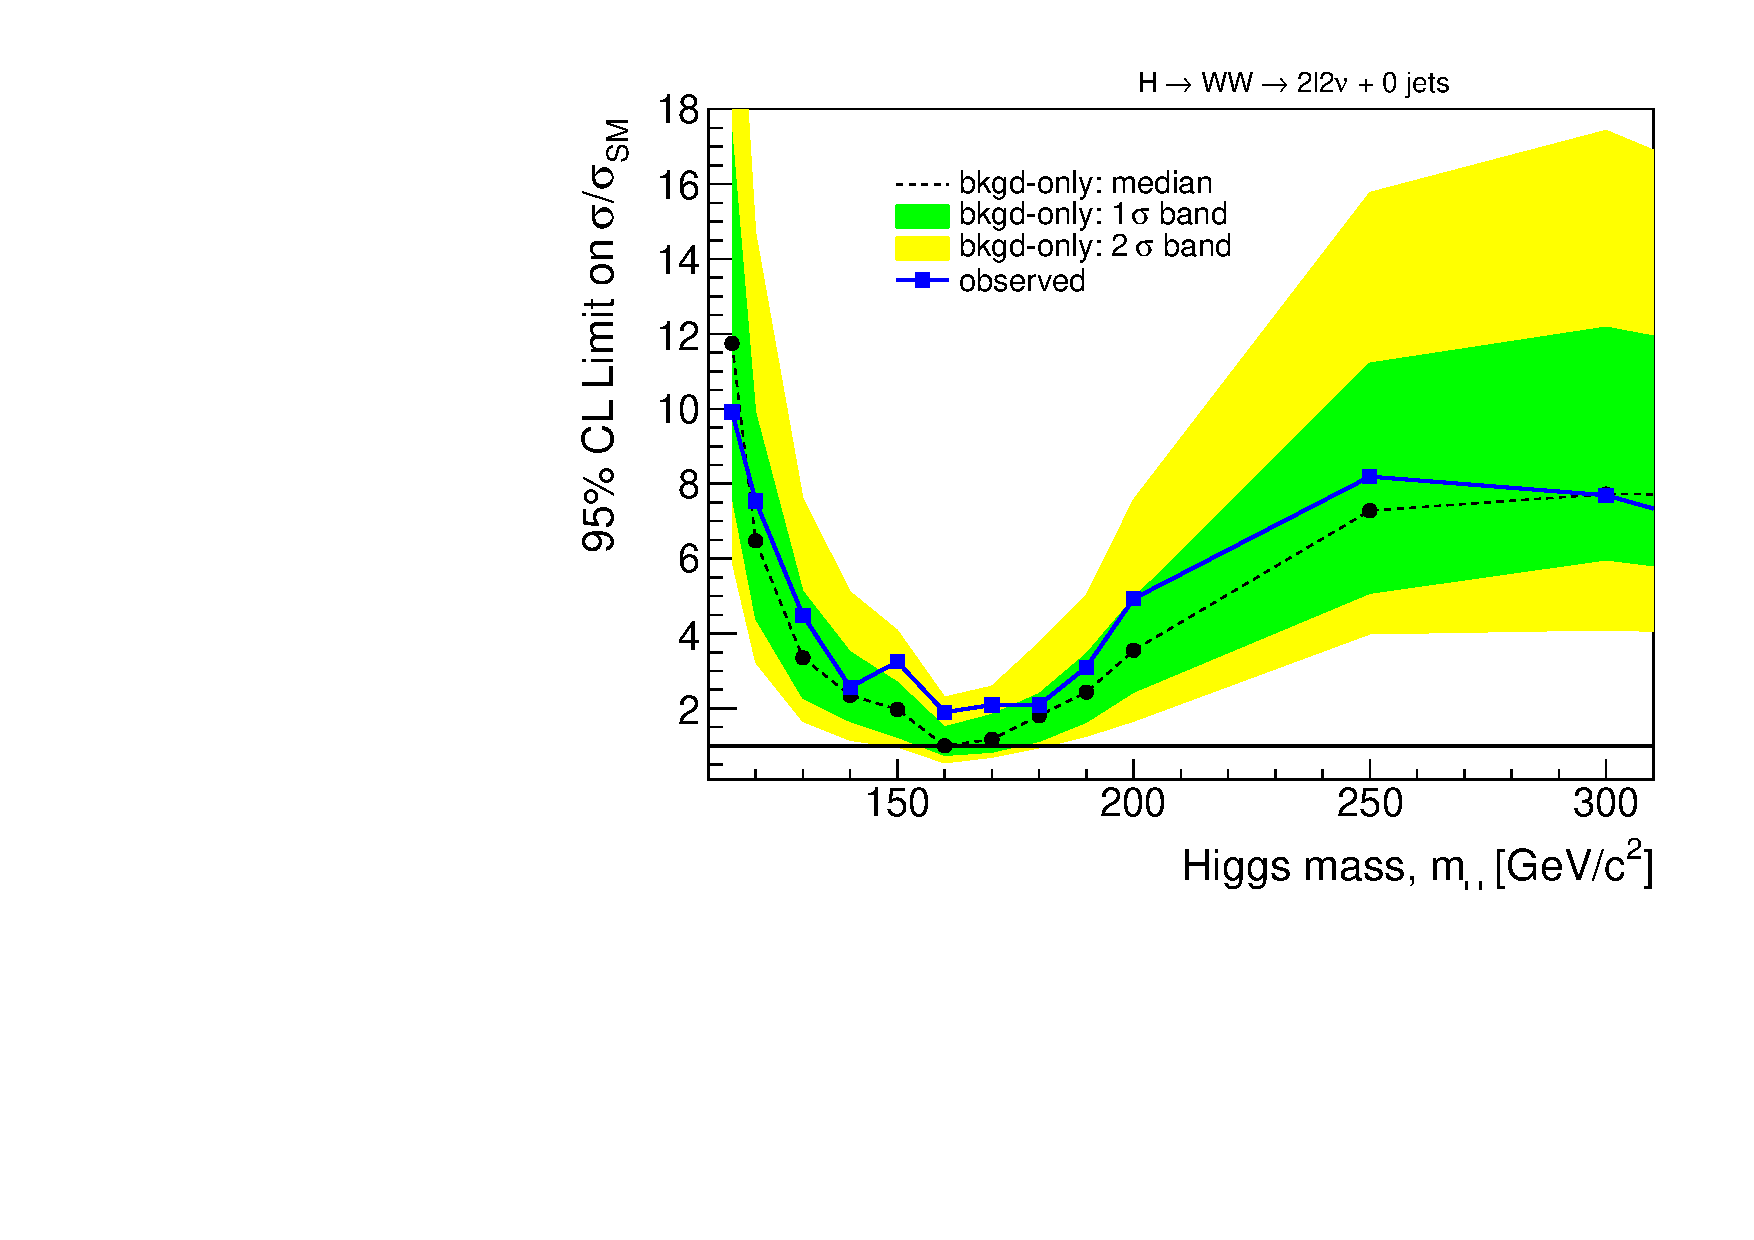
\includegraphics[width=0.49\textwidth]{figures/limits_0j_200pb_cut_1.pdf}
   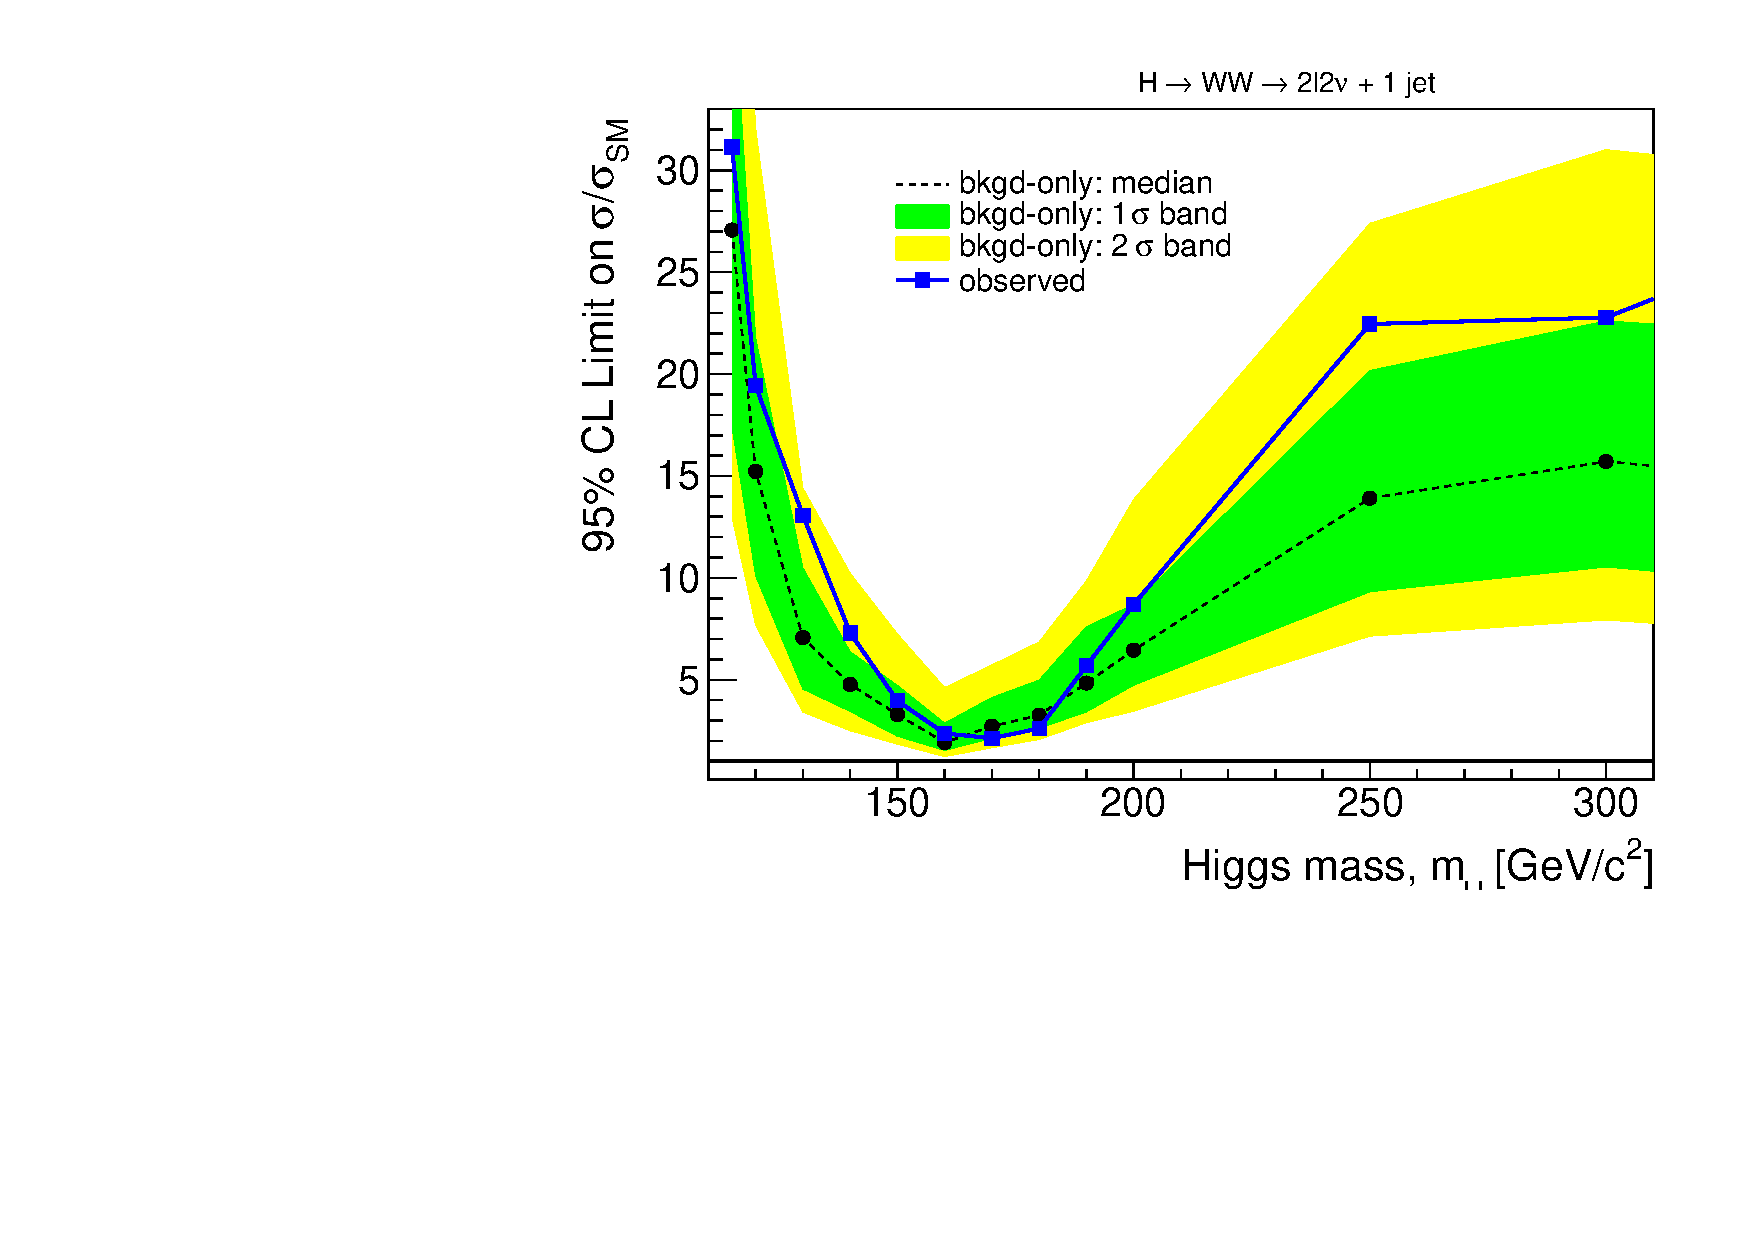
\includegraphics[width=0.49\textwidth]{figures/limits_1j_200pb_cut_1.pdf}
   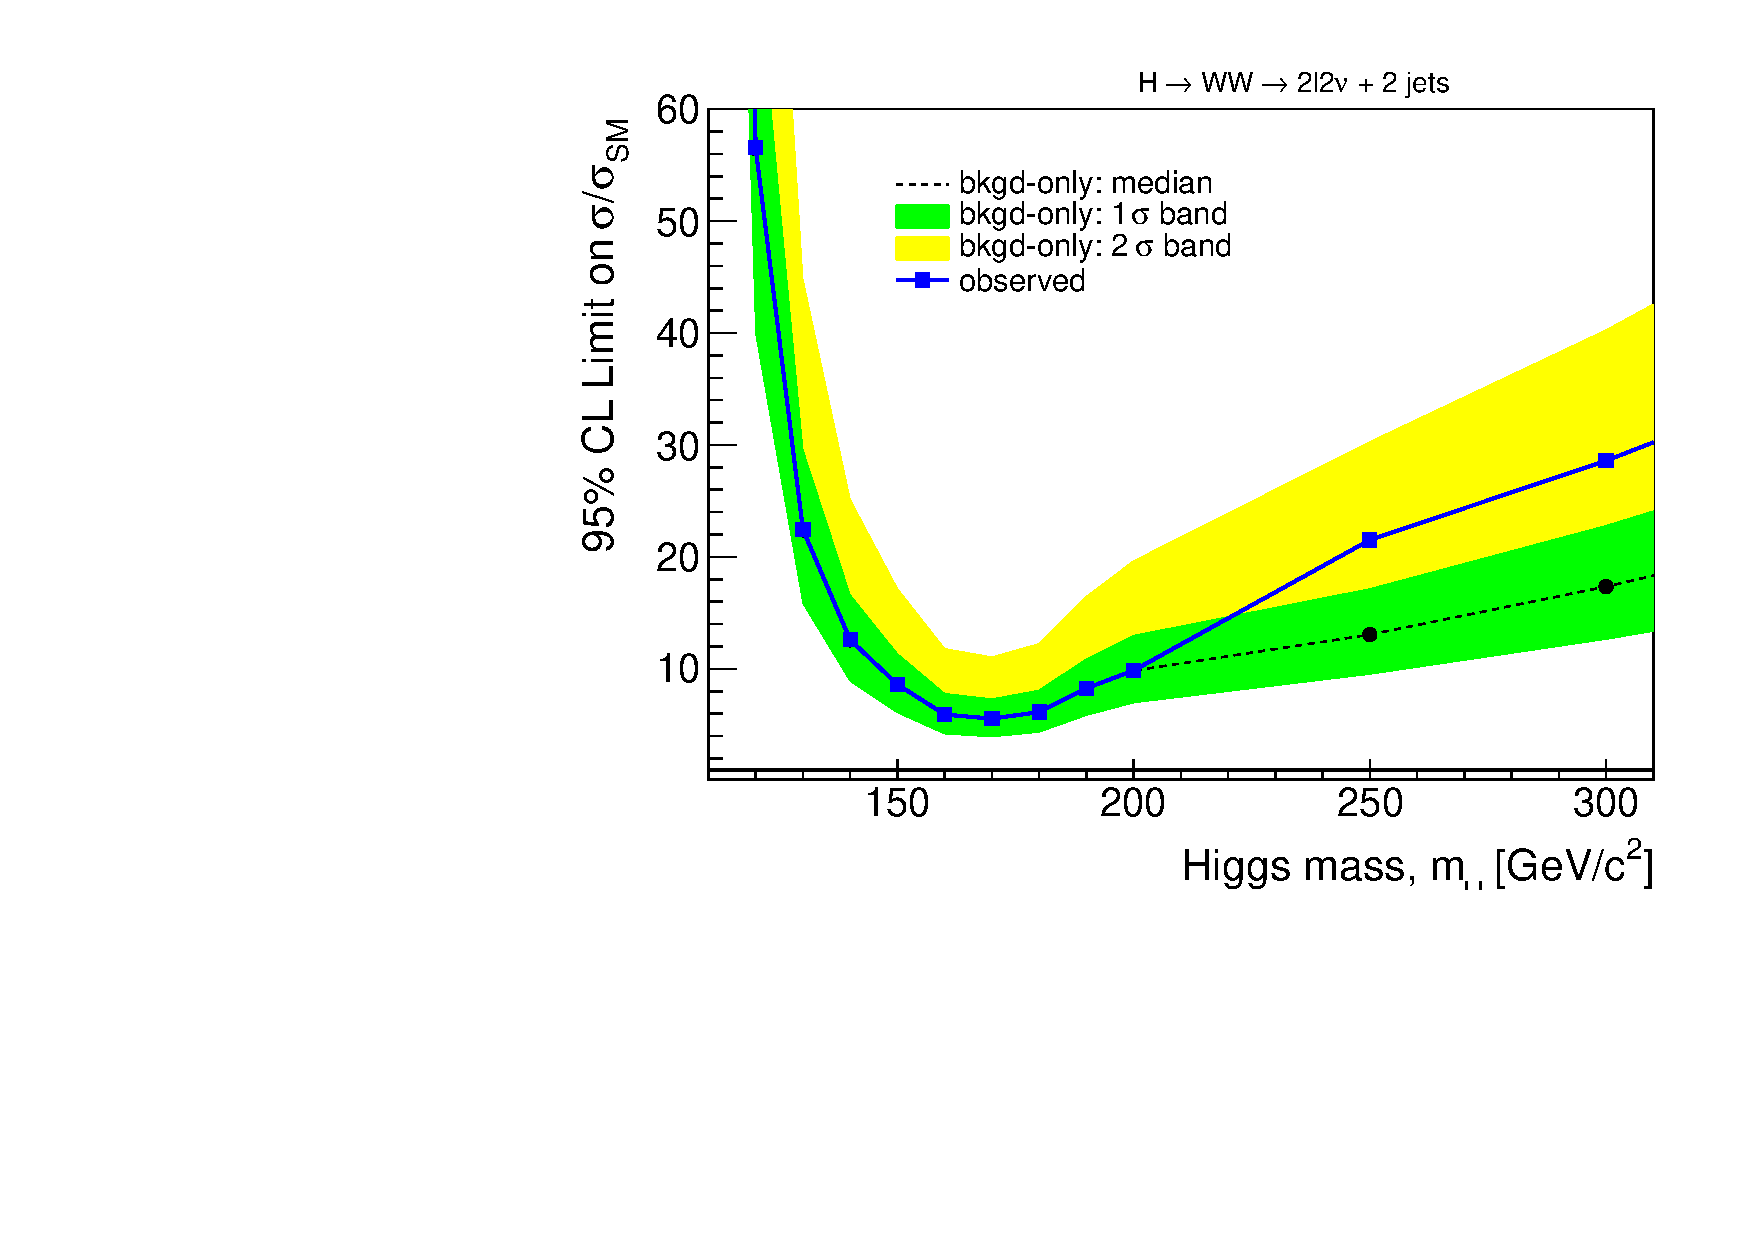
\includegraphics[width=0.49\textwidth]{figures/limits_2j_200pb_cut_1.pdf}
   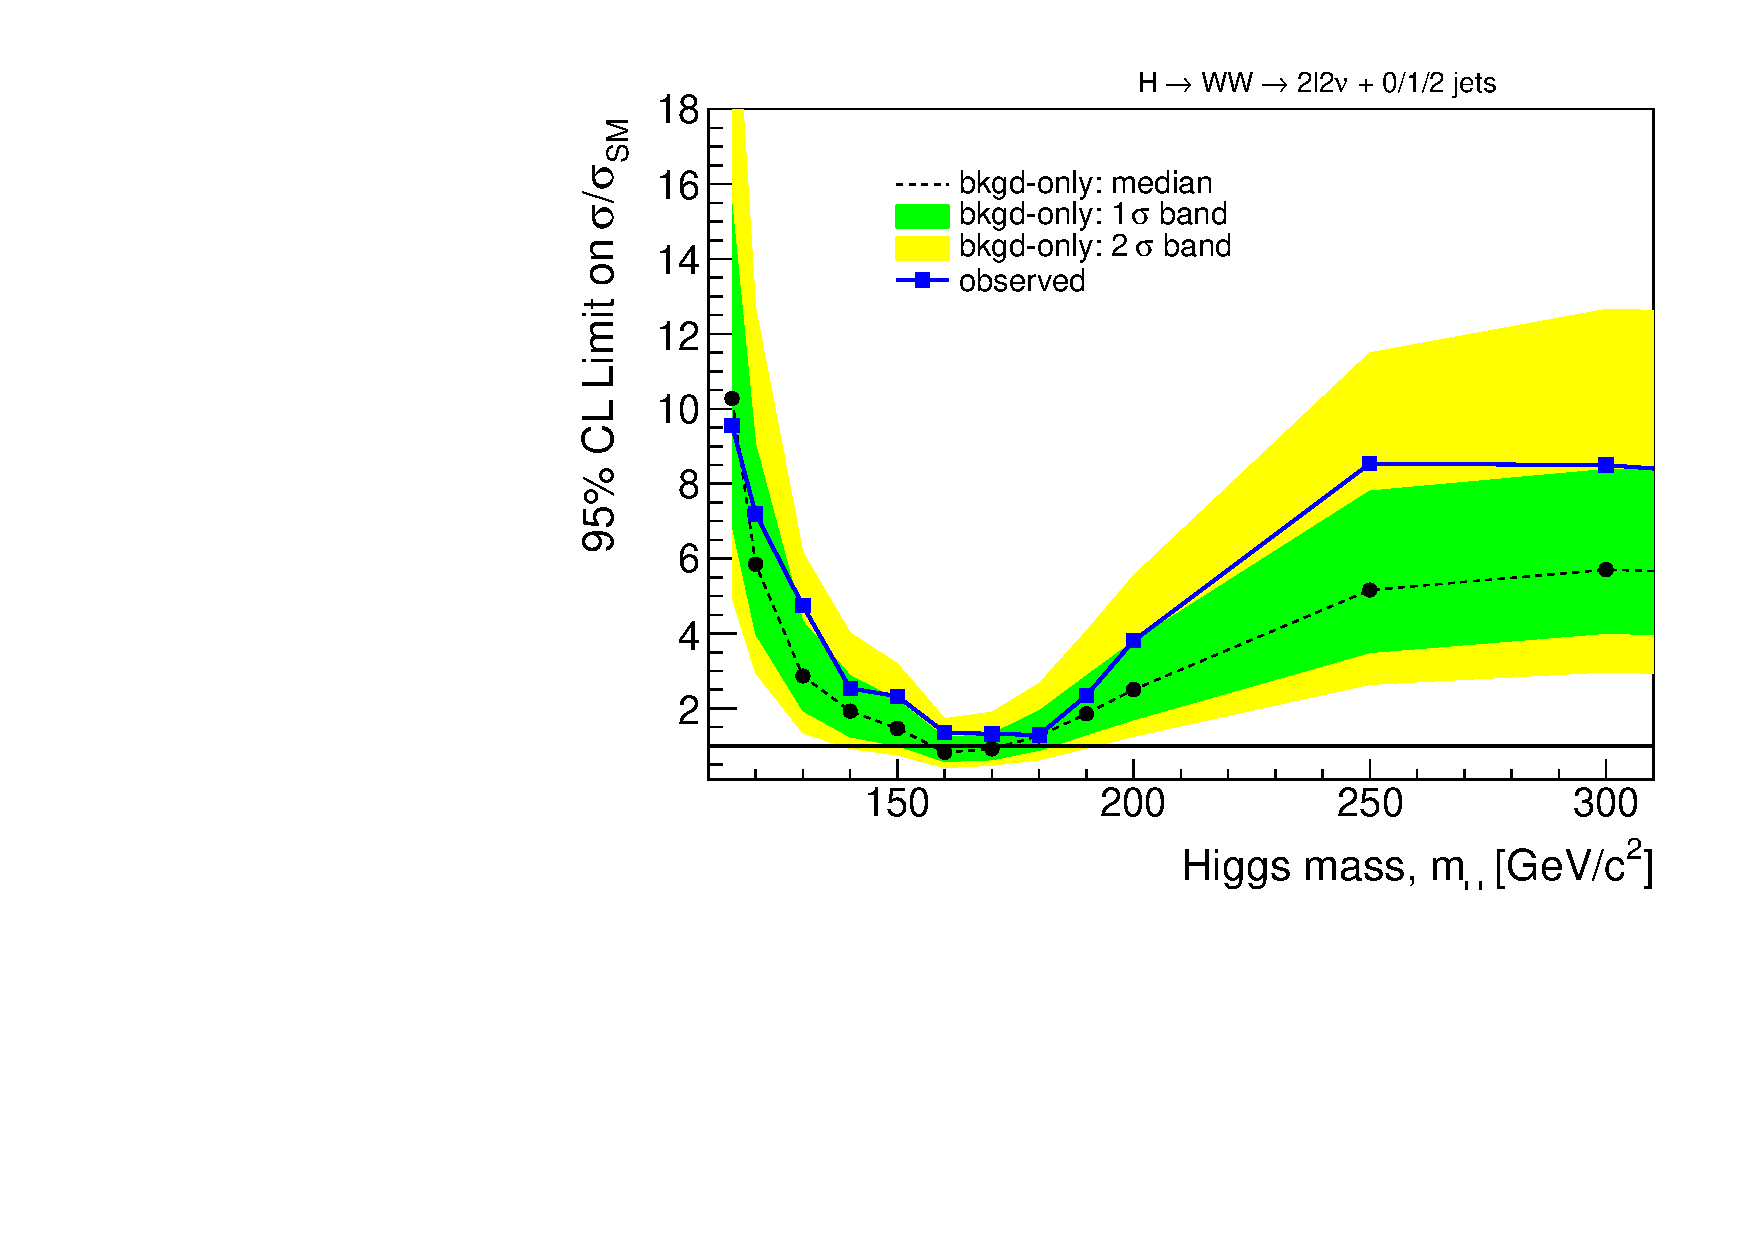
\includegraphics[width=0.49\textwidth]{figures/limits_nj_200pb_cut_1.pdf}
   \caption{Cut based analysis upper limits at 95\% C.L. for 188 $\ipb$ of data. Top left plot 
   is the result for the 0-jet bin, top right plot is the result for the 1-jet bin, bottom left plot 
   is the result for the 2-jet bin and, bottom right plot is the combined result.}
   \label{fig:cutbase_uls_data}
\end{center}
\end{figure}

\begin{figure}[!htbp]
\begin{center}
   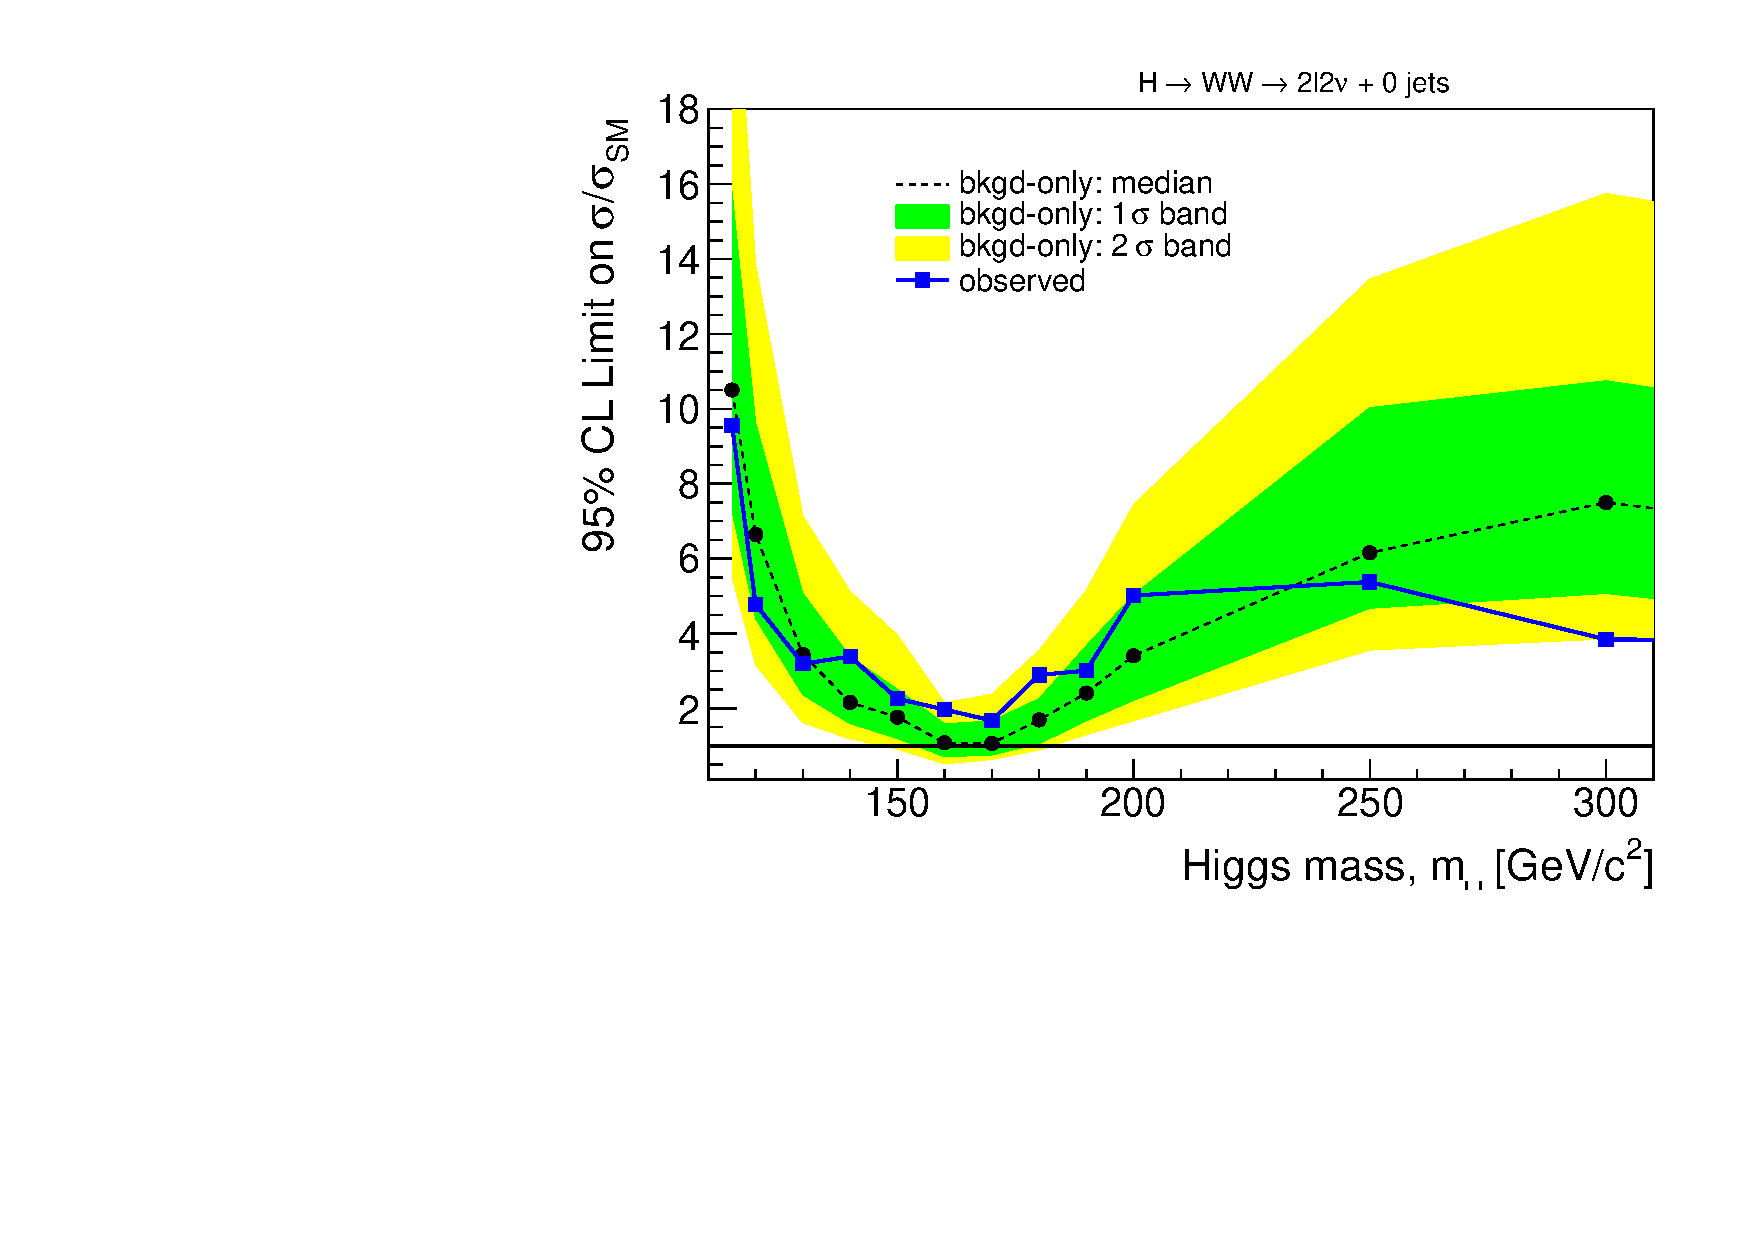
\includegraphics[width=0.49\textwidth]{figures/limits_0j_200pb_mva_1.pdf}
   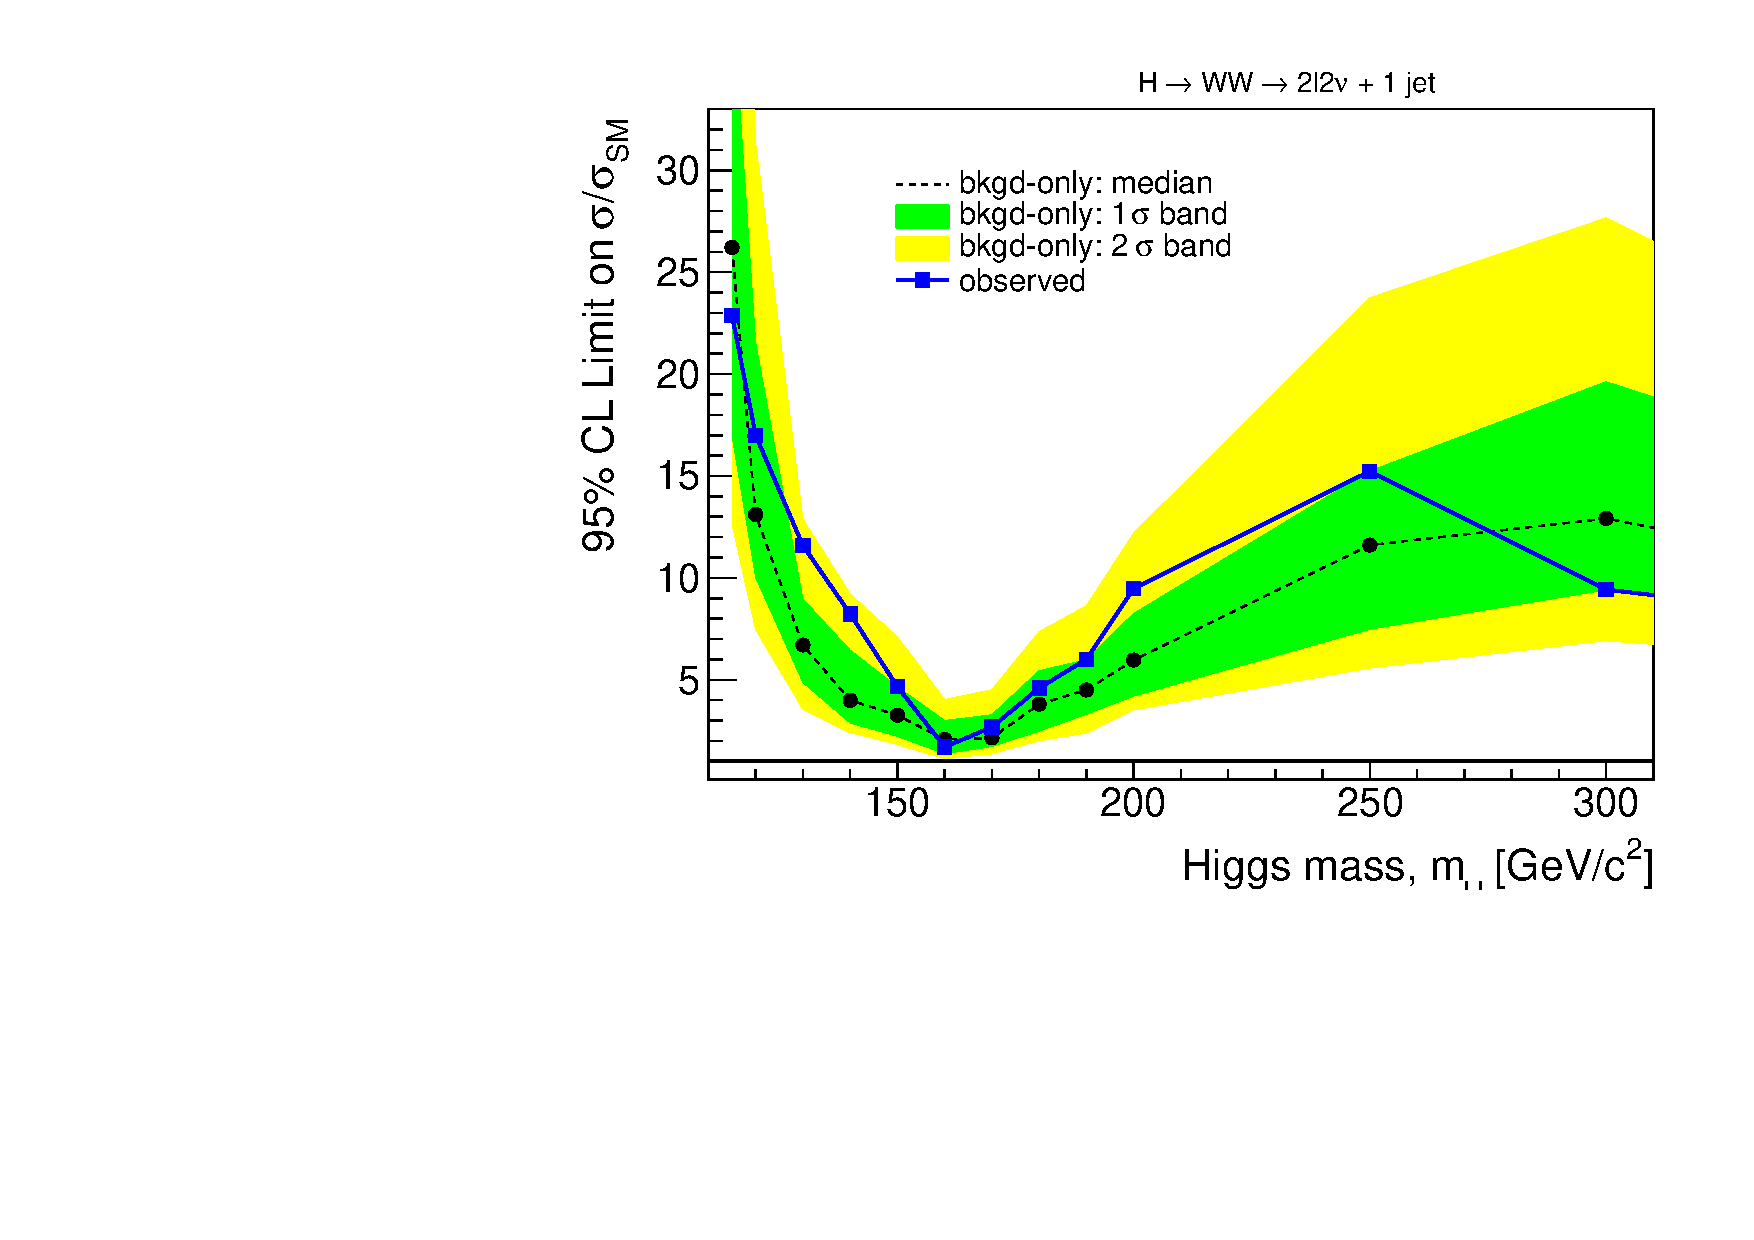
\includegraphics[width=0.49\textwidth]{figures/limits_1j_200pb_mva_1.pdf}
   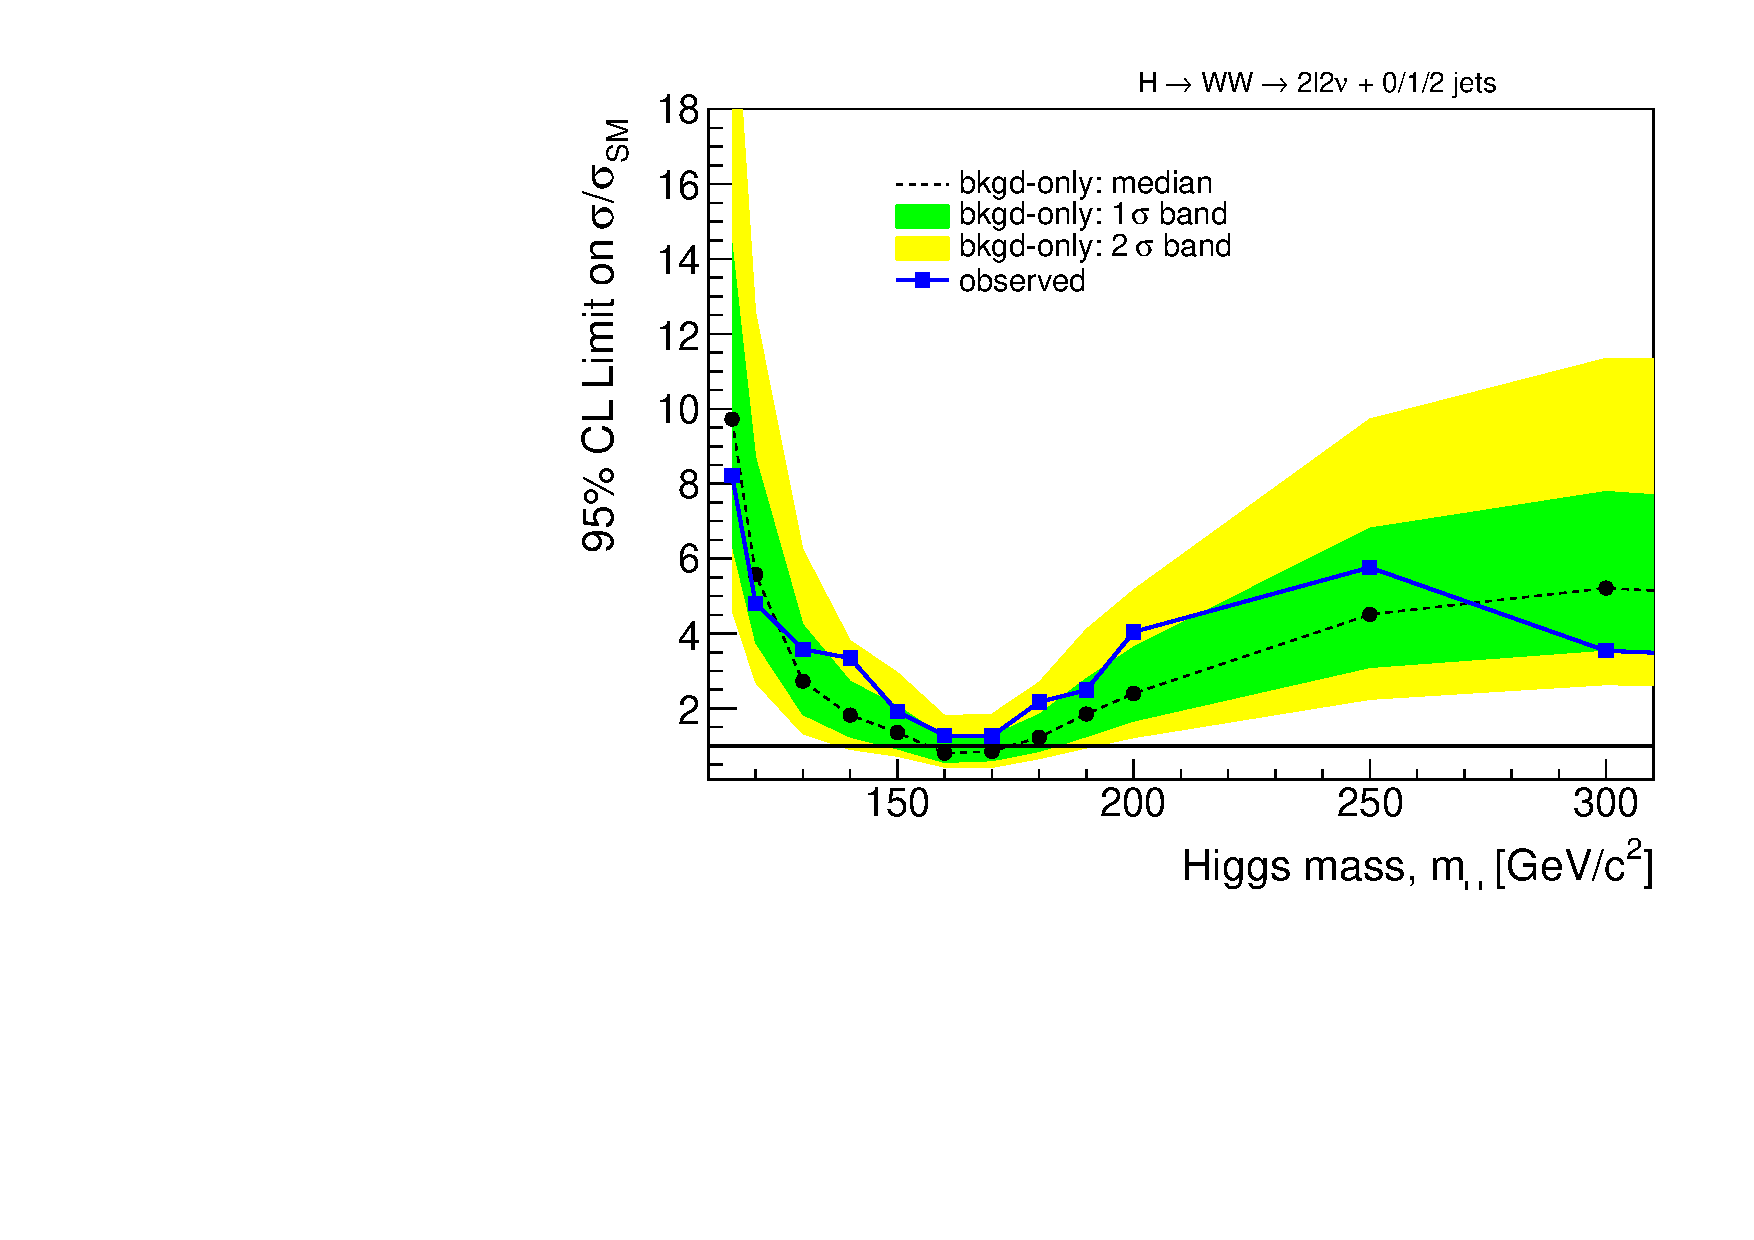
\includegraphics[width=0.49\textwidth]{figures/limits_nj_200pb_mva_1.pdf}
   \caption{Multivariate analysis upper limits at 95\% C.L. for 188 $\ipb$ of data. Top left plot 
   is the result for the 0-jet bin, top right plot is the result for the 1-jet bin and, 
   bottom right plot is the combined result.}
   \label{fig:mvabase_uls_data}
\end{center}
\end{figure}

\begin{figure}[!htbp]
\begin{center}
   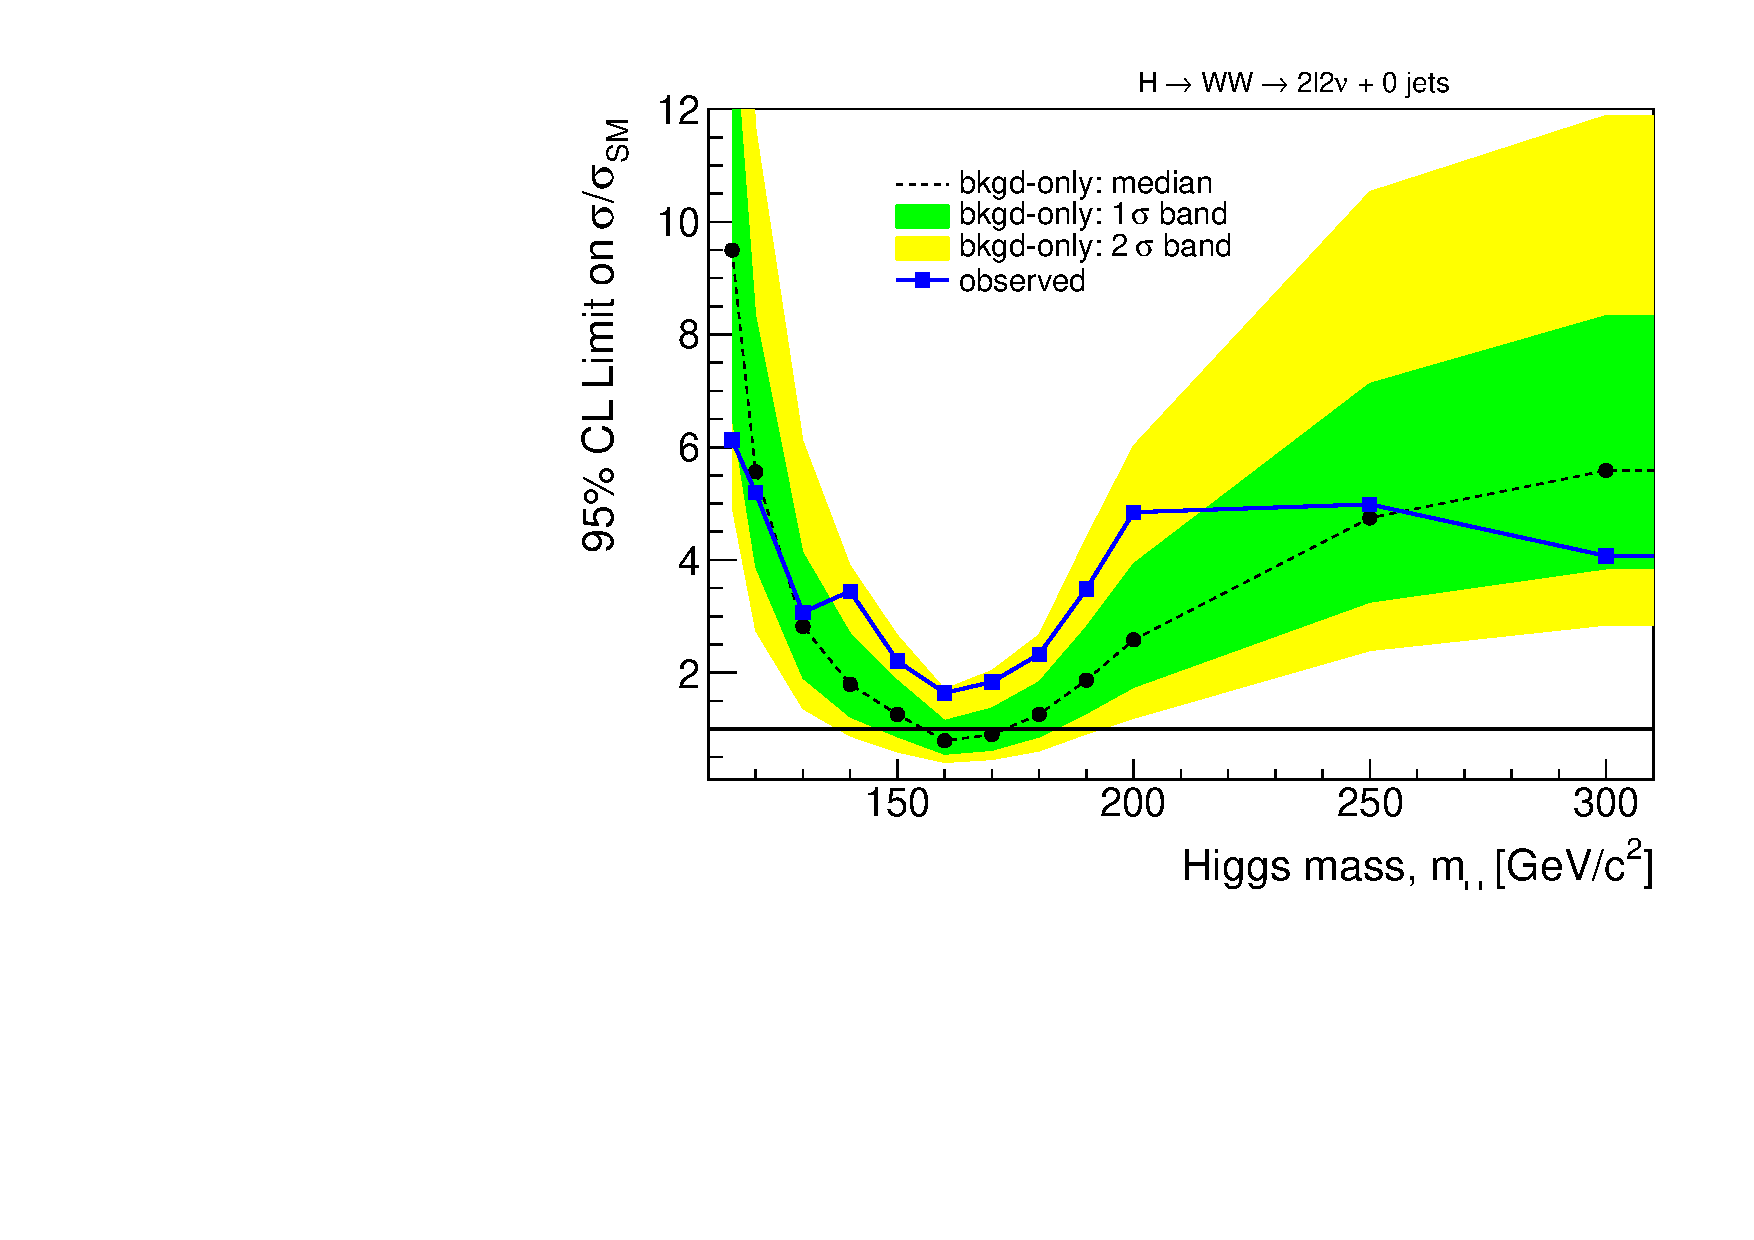
\includegraphics[width=0.49\textwidth]{figures/limits_0j_200pb_shape_1.pdf}
   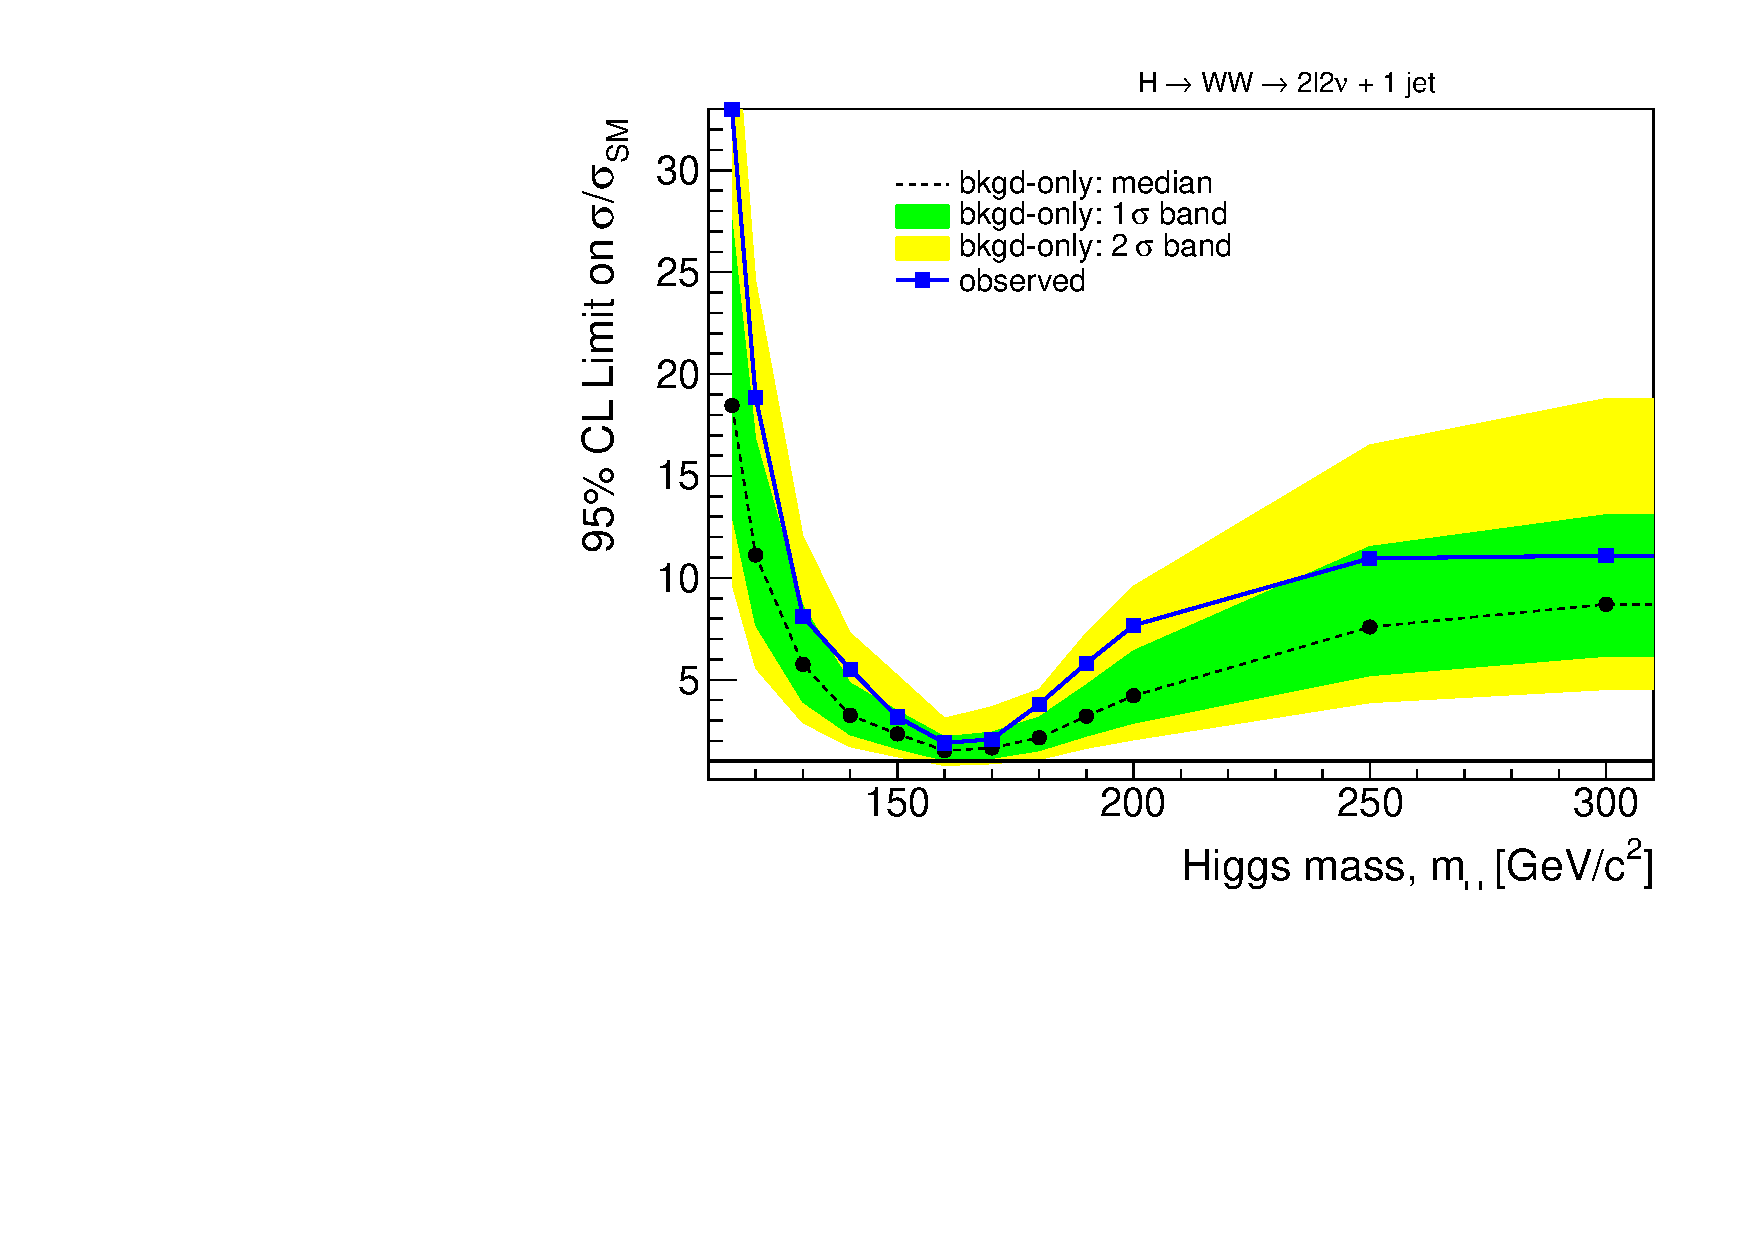
\includegraphics[width=0.49\textwidth]{figures/limits_1j_200pb_shape_1.pdf}
   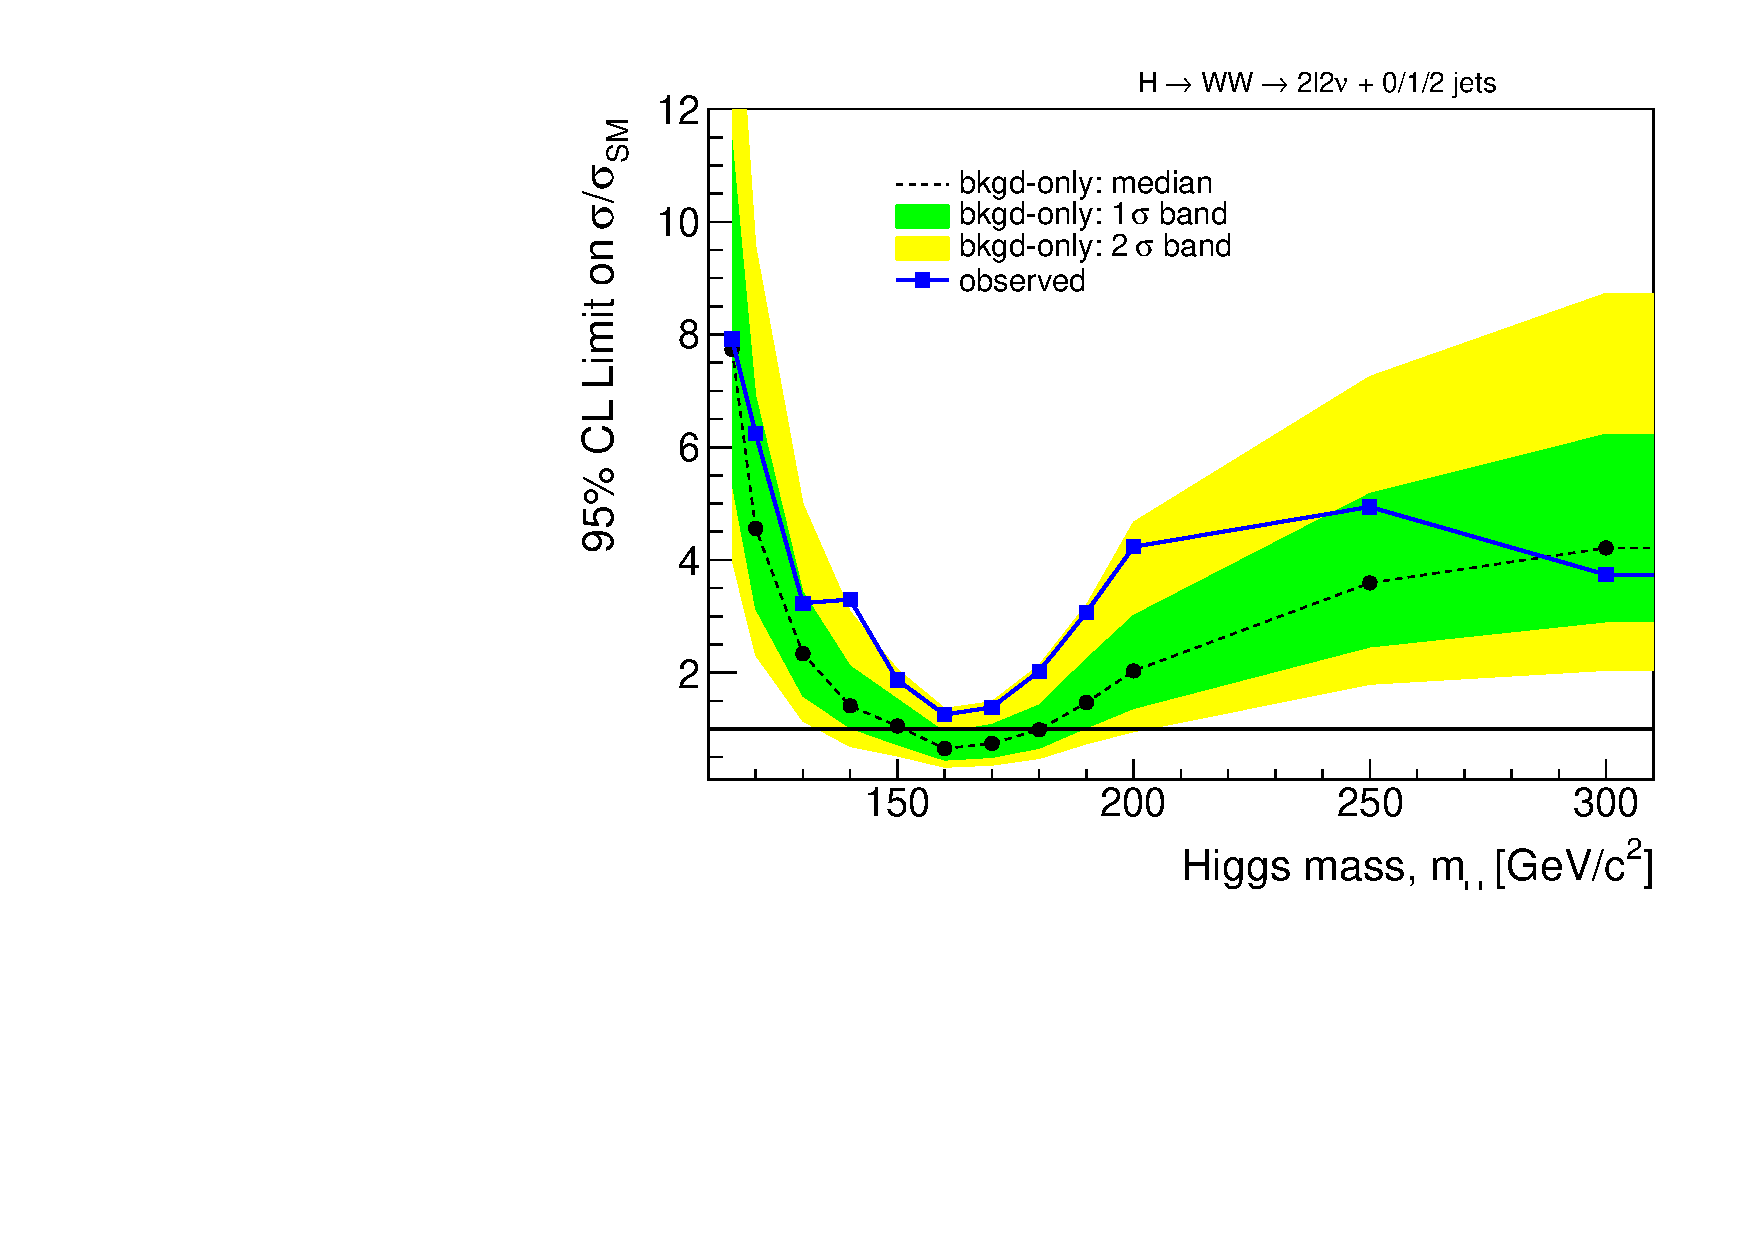
\includegraphics[width=0.49\textwidth]{figures/limits_nj_200pb_shape_1.pdf}
   \caption{Multivariate shape analysis upper limits at 95\% C.L. for 188 $\ipb$ of data. Top left plot 
   is the result for the 0-jet bin, top right plot is the result for the 1-jet bin and, 
   bottom right plot is the combined result.}
   \label{fig:mvashape_uls_data}
\end{center}
\end{figure}
